
\subsection{Critical Points and the Second Derivative Test}
To begin the process of optimization, we must first begin the same way we did in Calculus I. We wish to identify places where a surface has a maximum or minimum, i.e. the apex of a peak or bottom of a valley. To do so, we must identify critical points. In Calculus I, the critical points were the places where the derivative could change signs, that is, the derivative was zero or did not exist. We expand this idea. But first, lets introduce a useful characterization of the partial derivatives of a surface $f$: the \textbf{gradient}.

\begin{definition}{Gradient}
Let $f(\vcx)$ be a function $f:D\to \bbr$ where $D$ is a subset of $\bbr^n$. That is, $f$ is a function with an $n$-dimensional vector input. Then the \textbf{gradient} of $f(\vcx)$, written $\nabla f(\vcx)$ is defined as the $n$-dimensional vector:
$$\nabla f(\vcx)=\bmat{\frac{\del f}{\del x_1}\\ \frac{\del f}{\del x_2}\\ \vdots \\ \frac{\del f}{\del x_n}}. $$
In particular, if $f(x,y)$ is a surface in 3-d space, $$\nabla f(x,y)=\bmat{f_x\\f_y}.$$
\end{definition}

We then use the gradient to define our critical points.

\begin{definition}{Critical Points}
Let $f(x,y)$ be a differentiable surface. Then if $\nabla f(x_0,y_0)$ does not exist, or $\nabla f(x_0,y_0)=\vzero$, we say that $f(x,y)$ has a critical point at $(x_0,y_0)$.
\end{definition}

Much like in Calculus I, a critical point is necessary for a local maximum or minimum, but not sufficient. While we certainly have the same issues that arise from zeros where the derivative does not change sign, we also get a new issue, saddle points. 

\begin{example}{Critical Points}
Recall the function $f(x,y)=10-x^2+y^3-3y^2-6y$.
\vspace{1em}
\begin{center}
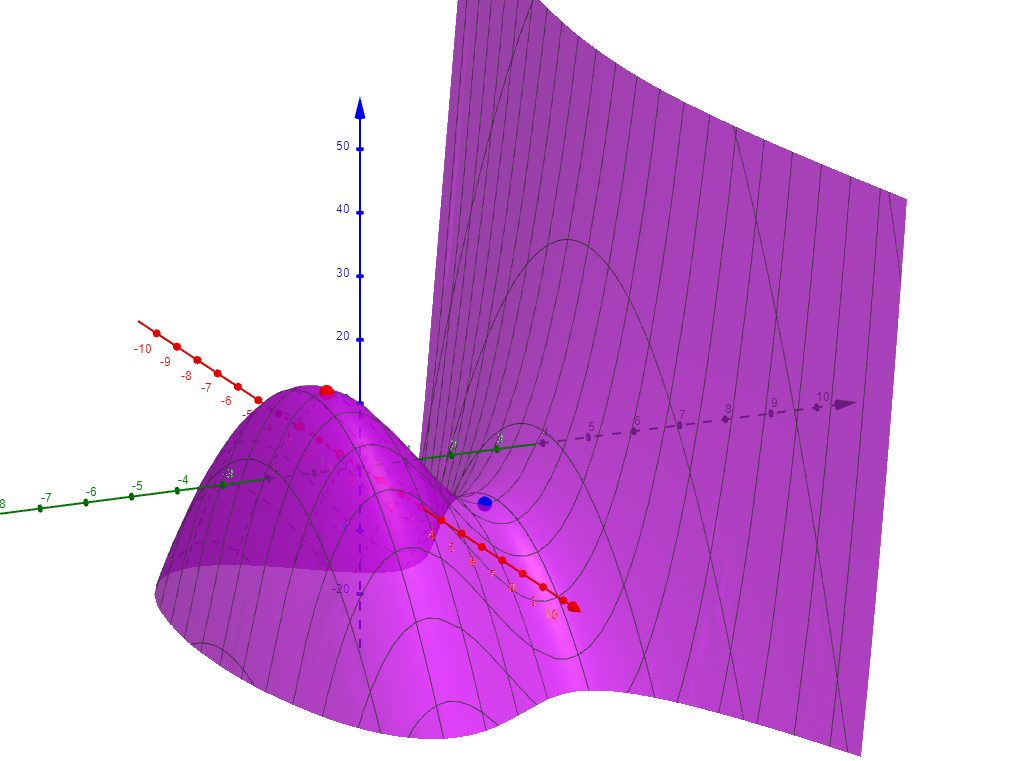
\includegraphics[scale=0.5]{Figures/surfaceex2} \\
 \href{https://www.geogebra.org/3d/ekkscrcb}{Geogebra Link to Graph}
\end{center}
Let's take our gradient:
$$\nabla f(x,y)=\bmat{-2x\\3y^2-6y-6} $$
Note that $\nabla f=0$ if $x=0$ and $y=1\pm\sqrt{3}$. This gives us two critical points, one at $(0,1+\sqrt{3})$ and the other at $(0,1-\sqrt{3})$. But looking at the graph, it is clear that $f$ has a local maximum at $(0,1-\sqrt{3})$ (the red dot), but at $(0,1+\sqrt{3})$ there is a \textbf{saddle point} (the blue dot).
\end{example}

\begin{exercise}{The Same Semi-sphere}
Consider, again, the function $$f(x,y)=\sqrt{16-x^2-y^2}.$$
Find the critical points of $f(x,y)$. You should find one point where $\nabla f=\vzero$, and an infinite family of points where $\nabla f$ doesn't exist.
\end{exercise}

You may recall that in Calculus I we had multiple ways of analytically categorizing critical points. In particular, we had a First Derivative Test (where we checked to see if the first derivative changed signs at our critical point), and a Second Derivative Test, where we checked the value of the second derivative. Unfortunately, there is no multivariate equivalent to the first derivative test. In particular, we would have to check every single possible path along the surface through our critical point to make sure that the derivative changed signs, which isn't really feasible. However, the second derivative test yields a multivariate version.

\begin{definition}{Second Derivative Test, Multivariable Edition}
Let $f(x,y)$ be a surface which has continuous second partials. Then define the discriminant, $$D(x,y)=f_{xx}f_{yy}-f_{xy}f_{yx}.$$ Note: Our condition here is the same as the Clairaut-Schwarz condition, so $f_{xy}=f_{yx}$, and so our discriminant is often written: $$D(x,y)=f_{xx}f_{yy}-(f_{xy})^2.$$ Let $f$ have a critical point at $(x_0,y_0)$. Then:
\vspace{1em}
\begin{itemize}
\item If $D(x_0,y_0)<0$, $f$ has a saddle at $(x_0,y_0)$.
\vspace{1em}
\item If $D(x_0,y_0)=0$, the test gives no information.
\vspace{1em}
\item If $D(x_0,y_0)>0$ and $f_{xx}(x_0,y_0)>0$ (or $f_{yy}(x_0,y_0)>0$), $f$ has a local minimum at $(x_0,y_0)$.
\vspace{1em}
\item If $D(x_0,y_0)>0$ and $f_{xx}(x_0,y_0)<0$ (or $f_{yy}(x_0,y_0)<0$), $f$ has a local maximum at $(x_0,y_0)$.
\end{itemize}
\end{definition}

\begin{exercise}{Clarifying the Second Derivative Test}
If $D(x_0,y_0)>0$, then the second derivative test can either check $f_{xx}$ or $f_{yy}$ to categorize the extrema. These are interchangeable because if $f_{xx}(x_0,y_0)>0$, then $f_{yy}(x_0,y_0)>0$ also. Why? (hint: the discriminant being positive here matters!)
\end{exercise}

\begin{example}{The Same Old}
Again, recall $f(x,y)=10-x^2+y^3-3y^2-6y$. As before, this function has critical points at $(0,1-\sqrt{3})$ and $(0,1+\sqrt{3}$. Lets compute our second partials and apply the second derivative test.
\begin{align*}
f_{xx}(x,y)=&-2\\
f_{yy}(x,y)=&6y-6\\
f_{yx}(x,y)=f_{xy}(x,y)=&0.
\end{align*}
Then \begin{align*}
D(x,y)=&(-2)(6y-6)-(0)(0)\\
=&-12y+12
\end{align*}
Note that it's often easier to evaluate the individual second derivatives rather than finding an explicit expression for $D(x,y)$. Let's go ahead and plug in our two critical points:
\begin{align*}
D(0,1-\sqrt{3})=&-12(1-\sqrt{3})+12\\
=&-12+12\sqrt{3}+12\\
=&12\sqrt{3}.\\
D(0,1+\sqrt{3})=&-12(1+\sqrt{3})+12\\
=&-12-12\sqrt{3}+12\\
=&-12\sqrt{3}.
\end{align*}
Since $D(0,1+\sqrt{3})<0$, $f$ has a saddle point at $(0, 1+\sqrt{3})$. On the other hand, since $D(0,1-\sqrt{3})>0$ and $f_{xx}(0,1-\sqrt{3})=-2<0$, $f$ has a local maximum at $(0, 1-\sqrt{3})$, which confirms our observations from the graphs above.
\end{example}

\begin{exercise}{The Semi-sphere... Again}
Consider, yet again, the surface $$f(x,y)=\sqrt{16-x^2-y^2}.$$ You found critical points earlier. The points where the partials don't exist defy the second derivative test, but you can use the second derivative test on the other critical point to categorize it.
\end{exercise}

\begin{exercise}{Finding Extrema}
Consider the surface $f(x,y)=x^2+xy+y^2-x+y+1$. Find all of the critical points of $f(x,y)$ and categorize them as saddles, minimums or maximums.
\end{exercise}

\begin{exercise}{I'm Sorry in Advance}
Consider the surface $$f(x,y)=x^3y^3-x^3y-xy^3+xy.$$
\begin{enumerate}
\item Take your partials and find all of the critical points of $f$. There should be \textit{thirteen}. (I told you I'm sorry! You may want to do some factoring by grouping.)
\vspace{1em}
\item Categorize each of the critical points as a saddle, minimum or maximum.
\vspace{1em}
\item Use the \href{https://www.geogebra.org/3d/nrqbqwen}{graph of the surface} to confirm your results from part 2.
\end{enumerate}
\end{exercise}
